% !TeX root = ../ejemplo.tex

\section{Desarrollo de la Aplicación Móvil}

Una aplicación móvil es un tipo de software diseñado para ejecutarse en dispositivos móviles, como teléfonos inteligentes o tabletas. A diferencia de las aplicaciones tradicionales para computadoras de escritorio, las aplicaciones móviles están optimizadas para operar con los recursos limitados de hardware de los dispositivos móviles, brindando funcionalidades específicas de manera eficiente. Aunque los dispositivos actuales son mucho más sofisticados que en sus primeras generaciones, las aplicaciones móviles siguen enfocándose en funciones concretas, permitiendo a los usuarios seleccionar solo las herramientas que necesitan en sus dispositivos \cite{IM1}.

Esta sección está enfocado en detallar el tipo de aplicación desarrollada para el proyecto, justificando las decisiones tecnológicas tomadas en cuanto a lenguajes, sistemas operativos y herramientas de desarrollo. Se explican los distintos tipos de aplicaciones móviles existentes, las razones detrás del uso de Kotlin y Android, así como las herramientas empleadas para su implementación.

\subsection{Tipos de aplicaciones móviles}
Existen diferentes tipos de aplicaciones móviles que responden a las necesidades y preferencias de los usuarios, así como a las capacidades técnicas de los dispositivos. A continuación, se detallan cada uno:

\begin{figure}[htbp]
	\begin{center}
		\fbox{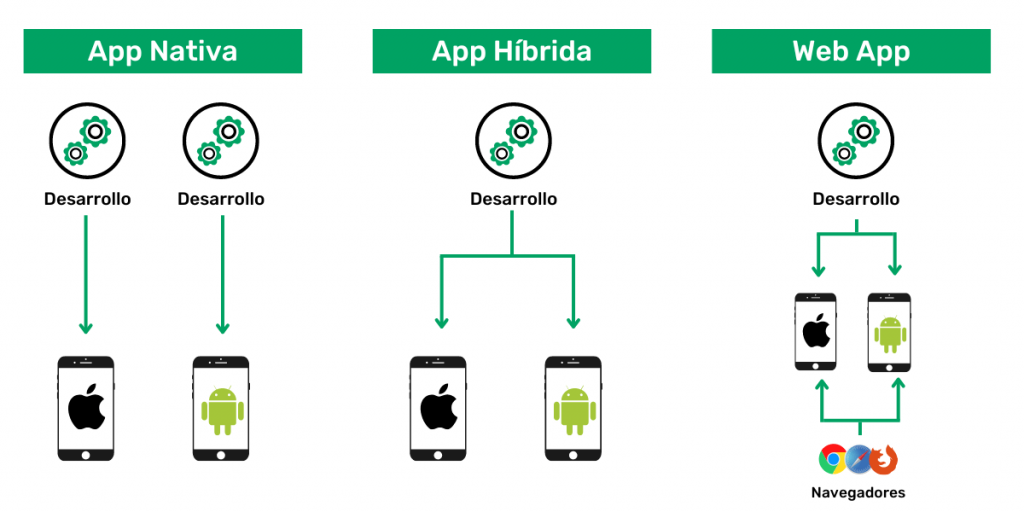
\includegraphics[width=.68\textwidth]{images/img08}}
		\caption{Tipo de aplicaciones moviles \cite{IM1}.}
		\label{fig:casosDeUso}
	\end{center}
\end{figure}

\subsection{Aplicaciones nativas}
Las aplicaciones nativas son apps desarrolladas para un sistema operativo móvil concreto (iOS o Android normalmente), en el lenguaje de programación específico de cada plataforma. Esto quiere decir que una app nativa creada para Android no puede ser utilizada en un dispositivo iOS y viceversa. \\

Es el tipo de aplicación móvil más conocida. Para que funcione, debemos descargarla desde los markets de apps, como App Store o Google Play e instalarla en nuestro teléfono \cite{CitaA02}.

\subsection*{Ventajas}
\begin{itemize}
	\item \textbf{Tienen el mejor rendimiento.} Las aplicaciones nativas son las más rápidas y tienen un rendimiento superior a otros tipos de apps, ya que han sido optimizadas específicamente para el hardware y el sistema operativo del dispositivo.
	\item \textbf{Acceso completo e integración con las funciones hardware del dispositivo.} Las apps nativas permiten aprovechar al máximo las funcionalidades móviles: cámara, micrófono, lector biométrico de huella, sensores y redes inalámbricas.
	\item \textbf{Pueden funcionar sin acceso a internet (funcionamiento offline)} si han sido diseñadas para ello.
\end{itemize}

\subsection*{Desventajas}
\begin{itemize}
	\item \textbf{Costes de desarrollo altos.} Si queremos tener nuestra app disponible para los dos sistemas, necesitaremos dos líneas de desarrollo diferentes, ya que el código utilizado para un sistema no es reutilizable para otro.
	\item \textbf{Complejidad de desarrollo.} Necesitamos equipos expertos en el lenguaje específico de cada sistema. Por ejemplo, en Kotlin para Android y en Swift para iOS.
	\item \textbf{Tiempo de desarrollo superior.} El desarrollo puede tomar entre 4 a 6 meses.
\end{itemize}

\subsection{Aplicaciones Web}

Las aplicaciones web realmente son webs especiales diseñadas para navegadores móviles. A diferencia de las apps nativas o híbridas, no necesitan ser descargadas, ya que se accede a ellas desde un navegador web.

Emplean las mismas tecnologías de desarrollo que una web, como HTML, CSS o JavaScript. Así, estaríamos hablando de una web con apariencia de app, por lo que presentaría sus mismas limitaciones. Sin embargo, con la llegada del HTML5, se han conseguido salvar algunas limitaciones, como el acceso a algunas funciones del móvil (geolocalización, cámaras) \cite{IM1}.

\subsection*{Ventajas}
\begin{itemize}
	\item \textbf{Carácter multiplataforma.} Con una sola línea de desarrollo.
	\item \textbf{Fácil desarrollo.} Se emplean tecnologías ampliamente conocidas.
	\item \textbf{Tiempo y coste de desarrollo bajo.}
\end{itemize}

\subsection*{Desventajas}
\begin{itemize}
	\item \textbf{Acceso limitado a las funciones del dispositivo.}
	\item \textbf{No se pueden subir a las tiendas de aplicaciones.}
	\item \textbf{Diferentes experiencias de usuario.} Estas dependen del navegador utilizado.
	\item \textbf{Necesidad de conexión a Internet.} Incluso si se cuenta con un modo pensado para ello, es necesario para acceder a las posibles actualizaciones o para entrar por primera vez.
\end{itemize}

\subsection{Aplicaciones Híbridas}

Las aplicaciones híbridas o multiplataforma combinan elementos de las aplicaciones nativas y las aplicaciones web. Estas aplicaciones se desarrollan utilizando tecnologías web como HTML, CSS y JavaScript, pero se empaquetan en un formato que puede ser instalado en un dispositivo móvil como cualquier otra aplicación nativa. Por tanto, podemos obtener una aplicación para varias plataformas con un único desarrollo \cite{IM1}.

\subsection*{Ventajas}
\begin{itemize}
	\item \textbf{Menor coste.} Gracias al uso de lenguajes de programación más conocidos, con una mayor disponibilidad de profesionales en el mercado.
	\item \textbf{Carácter multiplataforma.} Con una sola línea de desarrollo.
	\item \textbf{Acceso a algunas funcionalidades del móvil.}
	\item \textbf{Reducción de los tiempos de desarrollo.} Generalmente, el tiempo de desarrollo se reduce a 3 meses.
	\item \textbf{Disponibilidad en markets.} Se pueden subir a los markets de aplicaciones, como App Store y Google Play.
\end{itemize}

\subsection*{Desventajas}
\begin{itemize}
	\item \textbf{Rendimiento inferior.} Su rendimiento es inferior al de una app nativa, suelen tener un tamaño considerable y, además, ser más lentas.
	\item \textbf{Acceso limitado a las funciones del dispositivo.}
\end{itemize}

\subsection{Aplicaciones Progresivas Web Apps (PWA)}

Las aplicaciones progresivas son un reciente avance de las Web Apps. Al igual que las Web Apps, son webs diseñadas para móviles, pero esta vez, sí pueden ser descargadas en el móvil como una aplicación más, aunque no es necesario para que ofrezcan un comportamiento similar al de una app nativa a través del navegador. \\

Las PWA adoptan un comportamiento más propio de aplicaciones nativas que de web, como el funcionamiento sin Internet, un mayor rendimiento o su funcionamiento en segundo plano. Sin embargo, como desventaja, seguimos contando con la imposibilidad de subirlas a los markets de aplicaciones \cite{IM1}. \\

Para comprender mejor las diferencias entre los tipos de aplicaciones móviles, a continuación se presenta una tabla comparativa que destaca sus características clave:
\newpage

\begin{table}[h!]
	\centering
	\begin{tabular}{|p{4cm}|p{2cm}|p{2cm}|p{2cm}|}
		\hline
		\textbf{Tipos de app} & \textbf{Nativa} & \textbf{Híbrida} & \textbf{Web} \\ \hline
		\textbf{Interfaz} & Basada en web & Específica de la plataforma (iOS, Android) & Basada en web \\ \hline
		\textbf{Tiempo de desarrollo} & Alto & Medio & Bajo \\ \hline
		\textbf{Coste de desarrollo} & Alto & Medio & Bajo \\ \hline
		\textbf{Multiplataforma} & No & Sí & Sí \\ \hline
		\textbf{Rendimiento} & Alto & Medio & Bajo \\ \hline
		\textbf{Acceso a los sensores del dispositivo} & Completo & Alto o Completo & Limitado \\ \hline
		\textbf{Tiendas de aplicaciones} & Sí & Sí & No \\ \hline
	\end{tabular}
	\caption{Comparación tipos de aplicaciones móviles. Elaboración propia}
	\label{tab:tipos_apps}
\end{table}

Para el desarrollo de nuestro trabajo terminal, hemos decidido optar por una aplicación híbrida con el uso de Kotlin. Esta decisión se basa en varios factores relacionados con los recursos disponibles, las características de nuestro público objetivo y los plazos establecidos. \\

La aplicación móvil está dirigida para estudiantes, alumnos y personal de seguridad de la Escuela Superior de Cómputo, donde la mayoría utiliza dispositivos con sistema operativo Android. La elección de una aplicación híbrida nos permite optimizar  la experiencia en Android, que es la plataforma que predomina entre nuestros usuarios. \\

Aunque las aplicaciones híbridas suelen desarrollarse con tecnologías web (como React Native o Flutter), para nuestro proyecto hemos decidido incorporar Kotlin para desarrollar modelos donde se requiera un rendimiento nativo o un acceso más profundo a las funciones del sistema operativo Android.Además, las aplicaciones híbridas permiten un desarrollo más rápido en comparación con las aplicaciones completamente nativas, ya que gran parte del código puede compartirse entre plataformas, así mismo, es una buena opción económica que se adapta a nuestro presupuesto \cite{IM1}. 